\documentclass[oneside]{article}
\usepackage[subtle]{savetrees}
\usepackage{wallpaper}
\usepackage{geometry}
\usepackage[
    unicode=true,
    bookmarks=true,
    bookmarksnumbered=false,
    bookmarksopen=true,
    bookmarksopenlevel=1,
    breaklinks=false,
    pdfborder={0 0 0},
    backref=false,
    colorlinks=false
    ]{hyperref}
\usepackage{lastpage}
\usepackage{hyphenat}
\usepackage{hyphsubst}
\usepackage{tabularx}
\usepackage{moresize}
\usepackage[document]{ragged2e}
% \usepackage{parskip}

\usepackage[scaled]{helvet}
\usepackage{fontawesome5}
\usepackage[defaultfam,tabular,oldstyle]{montserrat}
\usepackage[T1]{fontenc}
\renewcommand*\oldstylenums[1]{{\fontfamily{Montserrat-TOsF}\selectfont #1}}

\usepackage{titlesec}
\usepackage{xcolor}
\usepackage{tikz}

\setlength{\parindent}{0pt}
\titleformat{\section}{\normalfont}{}{0pt}{}

\renewcommand{\arraystretch}{1.4}

\setlength\fboxrule{0pt}
\setlength\fboxsep{12pt}
% \setlength{\parskip}{.5\baselineskip plus 2pt}
% \renewcommand{\baselinestretch}{1.1}

\titlespacing{\section}{0pt}{1.5ex plus .1ex minus .2ex}{1pc}

\newcolumntype{Y}{>{\RaggedRight\arraybackslash}X}

% Change PDF Meta Info here
\hypersetup{
    pdftitle={Luca Spanedda - CV - English},
    pdfauthor={Luca Spanedda},
    pdfsubject={CV}
}

% Paper size
\geometry{
    a4paper,
    left=0pt,
    right=0pt,
    top=0pt,
    bottom=0pt,
    nohead,
    % includefoot,
    nomarginpar
}

% Background Color of the Sidebar Column
\definecolor{sidebg}{cmyk}{.6, .4, .4, 1.0}
% Background Color of the Main Column
\definecolor{mainbg}{cmyk}{0, 0, 0.04, 0.04}

% Text Color of the Main Column
\definecolor{maintext}{cmyk}{.6, .4, .4, 1.0}
% Text Color of the Sidebar Column
\definecolor{sidetext}{cmyk}{0, 0, 0, 0}

\pagecolor{mainbg}

\begin{document}
\setlength{\topskip}{0pt}\setlength{\footskip}{0pt}%
\fcolorbox{red}{sidebg}{%
    \begin{minipage}[t][\textheight-2\fboxsep-2\fboxrule][t]{\dimexpr0.40\textwidth-2\fboxrule-2\fboxsep\relax}
        \color{sidetext}
        %%%%%%%%%%%%%%%%%%%%%%%%%%%%%%%%%%%%%%%%%%%%%%%%%%%%
        % YOUR NAME, PRONOUNS, OCCUPATION(s), AND HEADSHOT
        {\bfseries\scshape\HUGE Luca} \\
        {\bfseries\scshape\Huge Spanedda} \qquad {he/him}
        \vspace{.0cm} \\
        \begin{center}
            \begin{tikzpicture}
            \clip (0,0) circle (3cm) node[anchor=center] {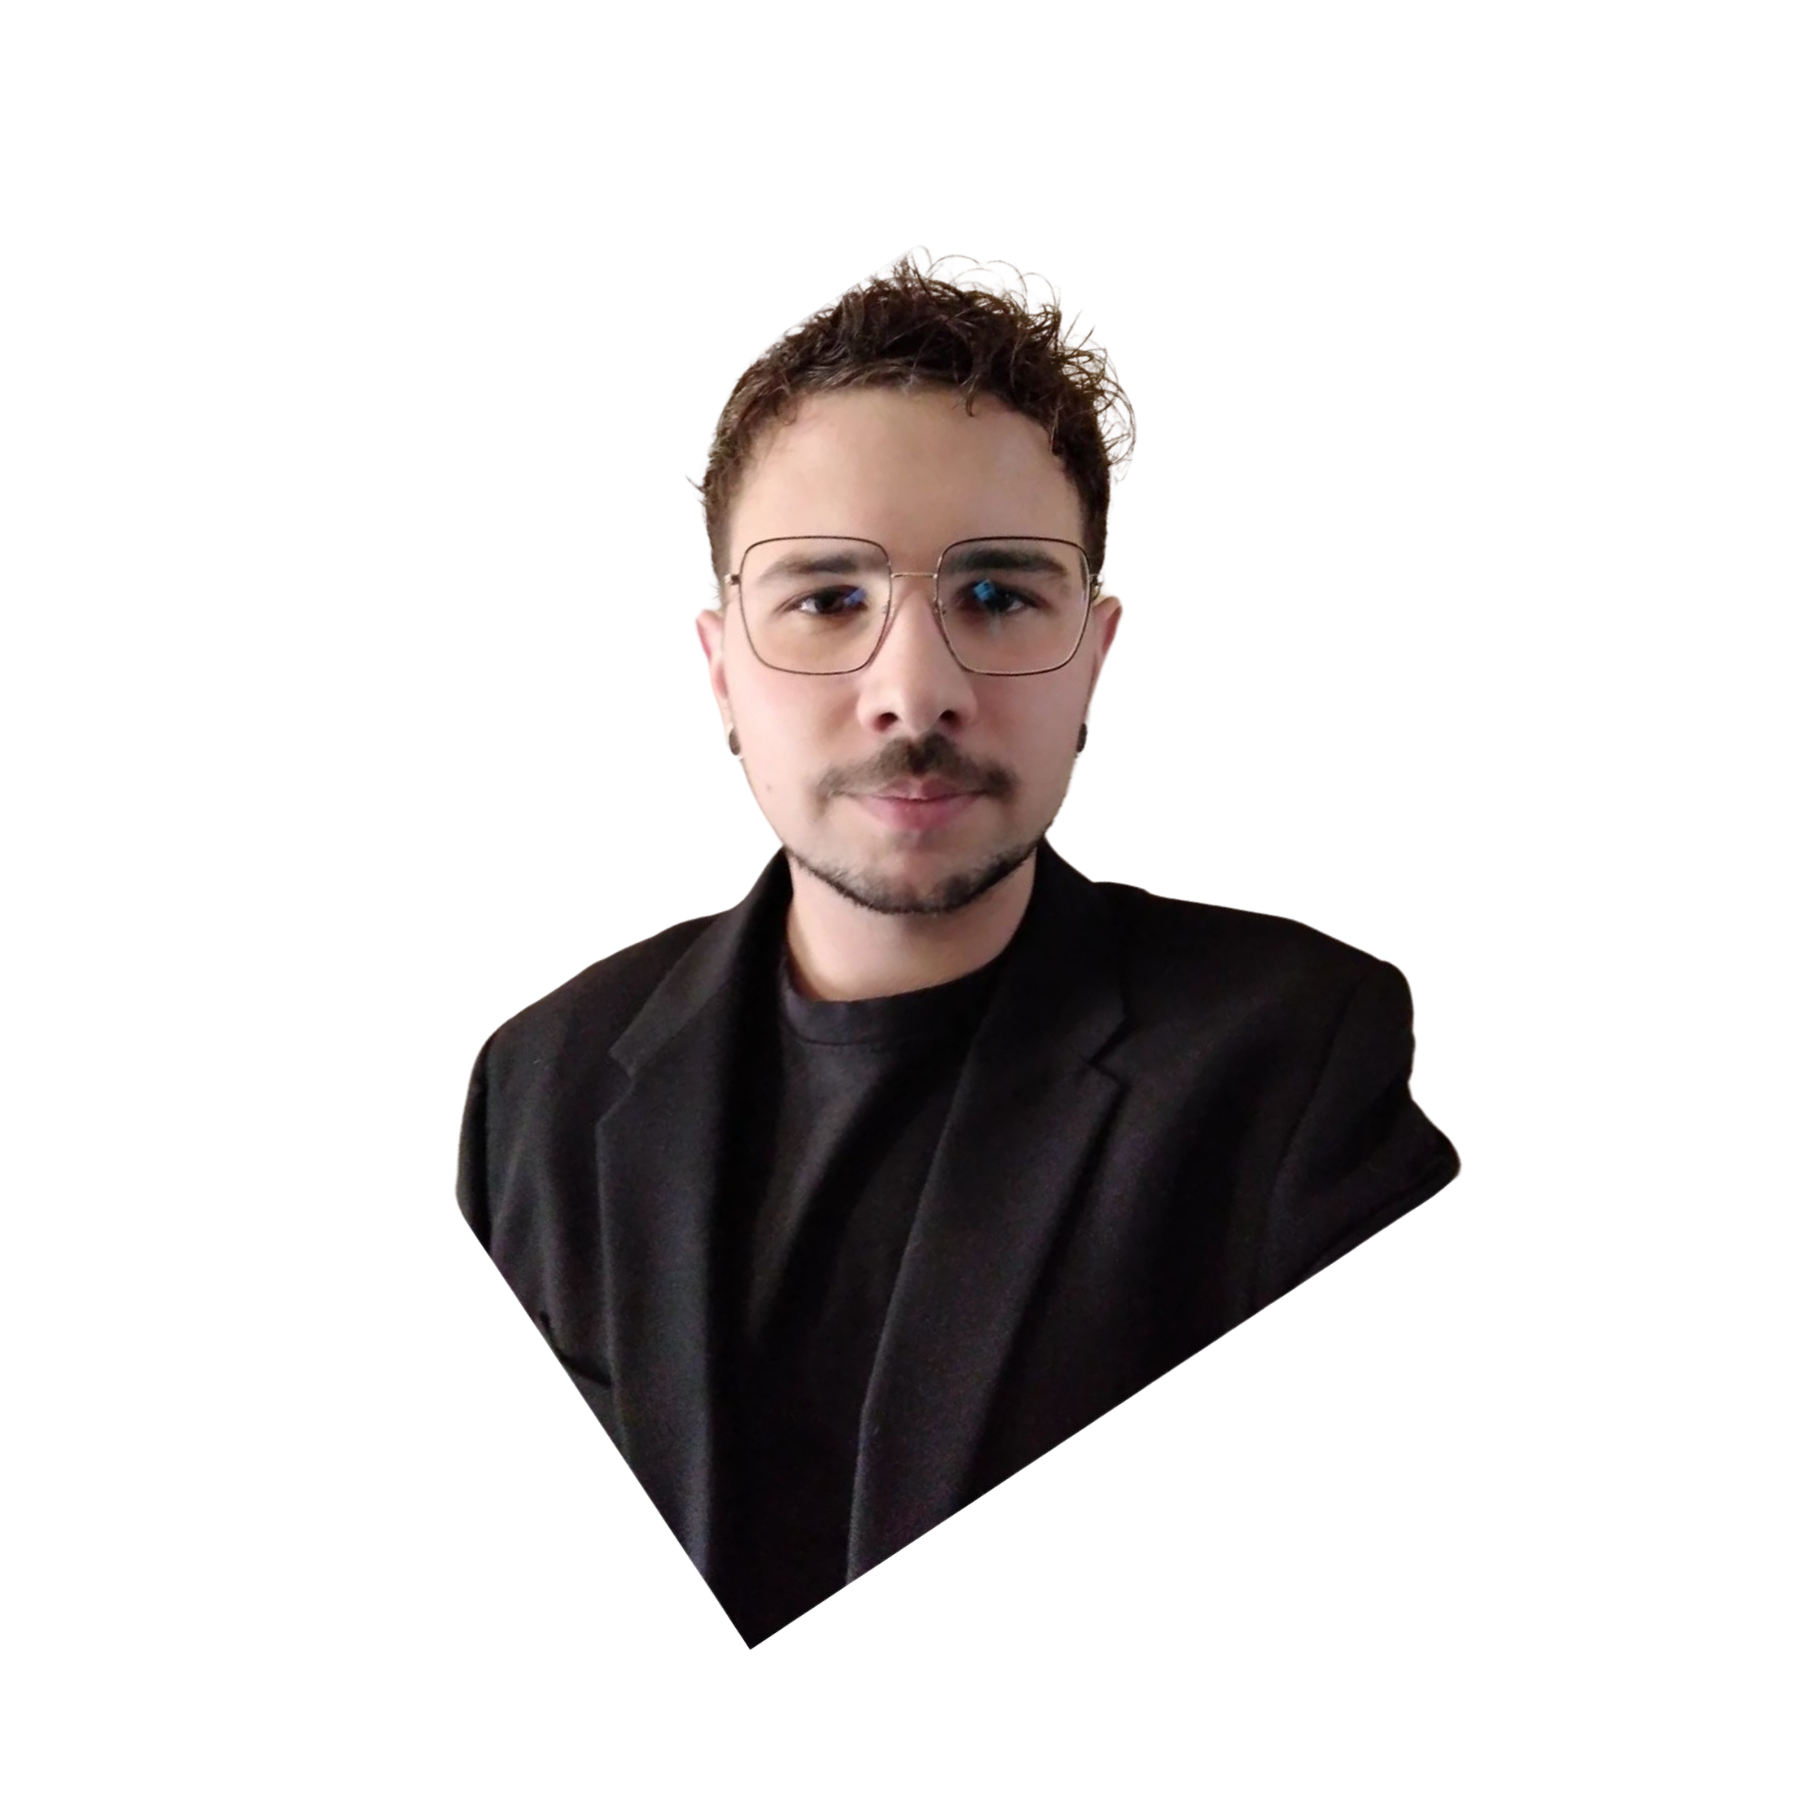
\includegraphics[width=6cm]{CV_Photo_align.png}}; 
            \end{tikzpicture}
        \end{center}
        \vspace{.2cm}
        %%%%%%%%%%%%%%%%%%%%%%%%%%%%%%%%%%%%%%%%%%%%%%%%%%%%
        % YOUR PERSONAL INFROMATION
        \phantomsection{}
        \addcontentsline{toc}{section}{Personal info}
        \section*{\large Personal info}
        \begin{tabularx}{\textwidth}{cY}
            \faStarOfLife{} & 15/02/1995 \\
            \faPhone{}      & +39-3663759122 \\
            \faEnvelope{}   & \href{mailto:lucaspanedda1995@gmail.com}{lucaspanedda1995@gmail.com} \\
            \faMapMarker{}  & Via Parigi 58, Ladispoli(RM), 00055, Italy \\
        \end{tabularx}
        \vspace{.3cm} \\
        \rule{\linewidth}{0.4pt} \\
        %%%%%%%%%%%%%%%%%%%%%%%%%%%%%%%%%%%%%%%%%%%%%%%%%%%%%%%%%
        % YOUR LINKS, YOU MAY ALSO ADD A PERSONAL WEBSITE OR PORTFOLIO
        \phantomsection{}
        \addcontentsline{toc}{section}{Links}
        \section*{\large Links}
        \begin{tabular}{cl}
        %    \faCode{}     & \href{https://example.com}{example.com}
            \faGithub{}   & \href{https://github.com/LucaSpanedda}{/LucaSpanedda} \\
            \faLinkedin{} & \href{https://www.linkedin.com/in/luca-spanedda/}{/luca-spanedda} \\
        \end{tabular}
        \vspace{10pt} \\
        \rule{\linewidth}{0.2pt} \\
        %%%%%%%%%%%%%%%%%%%%%%%%%%%%%%%%%%%%%%%%%%%%%%%%%%%%%%%%%%%%
        % YOUR SKILLS
        % Add/Remove as seen fit, Icons: https://packages.oth-regensburg.de/ctan/fonts/fontawesome5/doc/fontawesome5.pdf
        \phantomsection{}
        \addcontentsline{toc}{section}{Skills}
        \section*{\large Skills}
        \begin{tabularx}{\textwidth}{cY}
            \faCode{}        & Faust(GRAME), Pure Data, Max Msp, Csound, Python, Bash \\
            \faPen*{}        & \LaTeX, HTML, CSS \\
            \faFont{}        & \{MS, Libre, GSuite\} Office, Adobe Acrobat \\
            \faCogs{}        & Linux, Windows, macOS \\
        \end{tabularx}
        \vspace{1pt} \\
        \rule{\linewidth}{0.2pt}
        %%%%%%%%%%%%%%%%%%%%%%%%%%%%%%%%%%%%%%%%%%%%%%%%%%%%%%%%%%%%
        % EXPERTISE
        % Add/Remove as seen fit, Icons: https://packages.oth-regensburg.de/ctan/fonts/fontawesome5/doc/fontawesome5.pdf
        \phantomsection{}
        \addcontentsline{toc}{section}{Expertise}
        \section*{\large Expertise}
        \begin{tabularx}{\textwidth}{cY}
            \faAngleRight{} & \small composition for musical instruments, algorithmic composition, computer music, DSP
            programming, live electronics, embedded systems, autonomous installations, sound design, live recording,
            mixing, mastering. 
        \end{tabularx}
        \vspace{1pt} \\
        \rule{\linewidth}{0.2pt}
        %%%%%%%%%%%%%%%%%%%%%%%%%%%%%%%%%%%%%%%%%%%%%%%%%%%%%%%%%%%%
        % LANGUAGES
        \phantomsection
        \addcontentsline{toc}{section}{Languages}
        \section*{\large Languages}
        \begin{tabular}{cl}
            \faLanguage{} & Italian (Mothertounge) \\
            \faLanguage{} & English (Fluent)
        \end{tabular}
        \vspace{.2cm}
        \\
        \rule{\linewidth}{0.2pt}
        \vfill
    \end{minipage}
}
\hfill
\fcolorbox{red}{mainbg}{%
    \begin{minipage}[t][\dimexpr\textheight-2\fboxrule-2\fboxsep\relax][t]{\dimexpr0.6\textwidth-2\fboxrule-2\fboxsep\relax}
        \color{maintext}
        %%%%%%%%%%%%%%%%%%%%%%%%%%%%%%%%%%%%%%%%%%%%%%%%%%%%%%%%%%%
        % EDUCATION
        \phantomsection{}
        \addcontentsline{toc}{section}{Education}
        \section*{\scshape\Large Education \rule{\linewidth}{0.4pt}}
%
        {\large \textbf{Electronic Music, Santa Cecilia Conservatory of Music (Master's Degree)}} \\
        {\scshape\fontseries{light}\selectfont\footnotesize Rome \qquad Oct 2019 \textendash{} Mar 2023} \\
        \small
        {Degree: Second Level Academic Diploma} \\[1ex]
        {Grade: 110/110 cum laude} \\[1ex]
        {\footnotesize Thesis subject: Complex Adaptive Systems for Live Electronics musical performances} \\[2ex]

        {\large \textbf{Electronic Music, Santa Cecilia Conservatory of Music (Bachelor's degree)}} \\
        {\scshape\fontseries{light}\selectfont\footnotesize Rome \qquad Oct 2015 \textendash{} Jul 2020} \\
        \small
        {Degree: First Level Academic Diploma} \\[1ex]
        {Grade: 97/110} \\[1ex]
        {\footnotesize Thesis subject: The First Technical Figures in Electroacoustic Music} \\[2ex]

        {\large \textbf{Commercial Technical Education, High School ISIS Giuseppe Di Vittorio}} \\
        {\scshape\fontseries{light}\selectfont\footnotesize Ladispoli(RM) \qquad Aug 2015} \\
        \small
        {Degree: High School Diploma} \\[1ex]
        %%%%%%%%%%%%%%%%%%%%%%%%%%%%%%%%%%%%%%%%%%%%%%%%%%%%%%%%%%
        % Commissions
        \phantomsection{}
        \addcontentsline{toc}{section}{Commissions}
        \section*{\scshape\Large Commissions \rule{\linewidth}{0.4pt}}
%
        {\large \textbf{Waste Kompost Radio}} \\ 
        {{\fontseries{medium}\selectfont Project for Alan Alpenfelt, Daniela Allocca in collaboration with Pro Helvetia}} \\
        {\scshape\fontseries{light}\selectfont\footnotesize Apr 2023 \textendash{} Aug 2023} 
        \begin{itemize}
            \setlength{\itemsep}{-3pt}
            \small
            \item Algorithmic composer for a sound installation in collaboration with Dario Sanfilippo \\ 
            \vspace{.4cm}
                \begin{tabular}{cl}
                    %    \faCode{}     & \href{https://example.com}{example.com}
                        \faBook{} & \href{https://www.laregione.ch/culture/culture/1702511/radio-waste-kompost-suono-processo}{WKR on laRegione,} 
                        \href{https://www.luganolac.ch/it/lac/programma/evento~lac~23-24~s~fit~waste-kompost-radio~.html}{Lugano LAC,} 
                        \href{https://www.fitfestival.ch/eventi/waste-kompost-radio/}{FIT Festival} \\
                    \end{tabular}
            \end{itemize}
        %%%%%%%%%%%%%%%%%%%%%%%%%%%%%%%%%%%%%%%%%%%%%%%%%%%%%%%%%%%
        % COMPOSITIONS AND LIVE PERFORMANCES
        \phantomsection
        \addcontentsline{toc}{section}{Compositions and Live Performances}
        \section*{\scshape\Large Compositions and Live Performances \rule{\linewidth}{0.4pt}}
%
        \begin{justify}
            \setlength{\parindent}{0pt}
            {\large \textbf{RITI : Room Is The Instrument, at A.Casella Conservatory of L'Aquila}} \\
            {\scshape\fontseries{light}\selectfont\footnotesize \qquad Oct 2023} \\
            \small
            Performance in Live Electronics of RITI : Room Is The Instrument, at Temporary Concert Hall (LTCH) - Alfredo Casella Conservatory of L'Aquila 
        \end{justify}
            \begin{tabular}{cl}
                %    \faCode{}     & \href{https://example.com}{example.com}
                    \faBook{} & \href{https://www.ilmessaggero.it/abruzzo/conservatorio_aquila_rassegna-7669918.html}{elettroAQustica concert on il Messaggero} \\
                \end{tabular}

        \begin{justify}
            \setlength{\parindent}{0pt}
            {\large \textbf{Wires, at Conservatorio S.Cecilia in Rome - Sala Medaglioni}} \\
            {\scshape\fontseries{light}\selectfont\footnotesize \qquad Apr 2022} \\
            \small
            Performance by a string quintet of the composition "Wires" at Sala Medaglioni of the S.Cecilia Conservatory of Rome \\
            \end{justify}

        \begin{justify}
            \setlength{\parindent}{0pt}
            {\large \textbf{Live Electronics of Post-prae-ludium per Donau by Luigi Nono, at Goethe-Institut Italien in Rome}} \\
            {\scshape\fontseries{light}\selectfont\footnotesize \qquad Jul 2021} \\
            \small
            Performer for the Live Electronics parts in Post-prae-ludium per Donau by Luigi Nono, at Goethe-Institut Italien in Rome, Festival Arte e Scienza. \\
            \end{justify}

        \begin{justify}
            \setlength{\parindent}{0pt}
            {\large \textbf{Asteroids, at University of Rome "Tor Vergata" and Conservatorio S.Cecilia in Rome}} \\
            {\scshape\fontseries{light}\selectfont\footnotesize \qquad Jun 2017} \\
            \small
            Performance in Live Electronics of "Asteroids" Audio-Visual composition at the Master in Sonic Arts
            University of Rome "Tor Vergata" and at the academic hall of the S.Cecilia Conservatory in Rome. \\
            \end{justify}

        % \\
        \vfill%
        % {\hfill\small\fontseries{extralight}\selectfont Page \thepage of \pageref{LastPage}\hfill}
        \scriptsize I give consent to process my data with the purpose of the recruitment process, in accordance to the Regulation of the European
        Parliament 679/2016, regarding the protection of natural persons and free movement of such data.
    \end{minipage}
}%
\let\cleardoublepage\clearpage
\end{document}